\documentclass[aspectratio=169,11pt]{beamer}
\usepackage[T1]{fontenc}
\usepackage{booktabs}
\definecolor{ink}{HTML}{162C40}
\definecolor{accent}{HTML}{087F8C}
\definecolor{muted}{HTML}{526575}
\setbeamercolor{normal text}{fg=ink,bg=white}
\setbeamercolor{structure}{fg=accent}
\setbeamercolor{frametitle}{fg=ink}
\setbeamercolor{block title}{fg=white,bg=accent}
\setbeamercolor{block body}{fg=ink,bg=accent!7}
\setbeamerfont{frametitle}{size=\Large,series=\bfseries}
\setbeamertemplate{navigation symbols}{}
\setbeamertemplate{itemize items}[circle]
\setbeamertemplate{footline}{%
  \hspace{0.035\paperwidth}\textcolor{muted}{\scriptsize Salih Erdem Kaymak}\hfill
  \textcolor{muted}{\scriptsize\insertframenumber/\inserttotalframenumber}\hspace{0.035\paperwidth}\vspace{3mm}}
\setbeamersize{text margin left=9mm,text margin right=9mm}
\setlength{\parskip}{5pt}

\begin{document}

\begin{frame}[plain]
\vfill
{\LARGE\bfseries Sentiment-Aware CLIP Attributes for\\[2mm]
Hierarchical Multimodal Sarcasm Detection\par}
\vspace{9mm}
{\large Salih Erdem Kaymak\par}
{\large Student number: 26587006\par}
\vspace{5mm}
{\color{muted} Y{\i}ld{\i}z Technical University\\
Artificial Intelligence and Data Engineering\par}
\vfill
\end{frame}

\begin{frame}{Why multimodal sarcasm detection?}
\vspace{2mm}
\begin{columns}[c,onlytextwidth]
\begin{column}{0.43\textwidth}
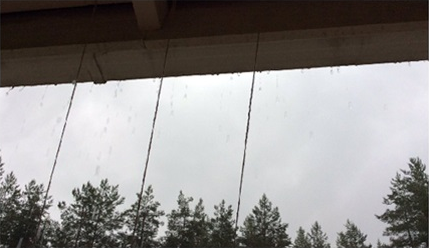
\includegraphics[width=\linewidth]{figures/cai2019_weather_example.png}
\begin{center}
\small ``What a wonderful weather!''
\end{center}
\end{column}
\begin{column}{0.54\textwidth}
\small
\begin{itemize}
  \item Sarcasm can lie in the \textbf{contrast between text and image}.
  \item I chose this topic to study how the two inputs interact.
  \item Research question: can \textbf{affective image descriptions} help?
\end{itemize}
\end{column}
\end{columns}
\vfill
{\scriptsize English tweet--image pairs from MMSD; binary sarcasm classification.\\
Example image and tweet: Cai et al., ACL 2019, Fig.~1(a).}
\end{frame}

\begin{frame}{Why reproduce Cai et al.'s HFM?}
\begin{columns}[c,onlytextwidth]
\begin{column}{0.69\textwidth}
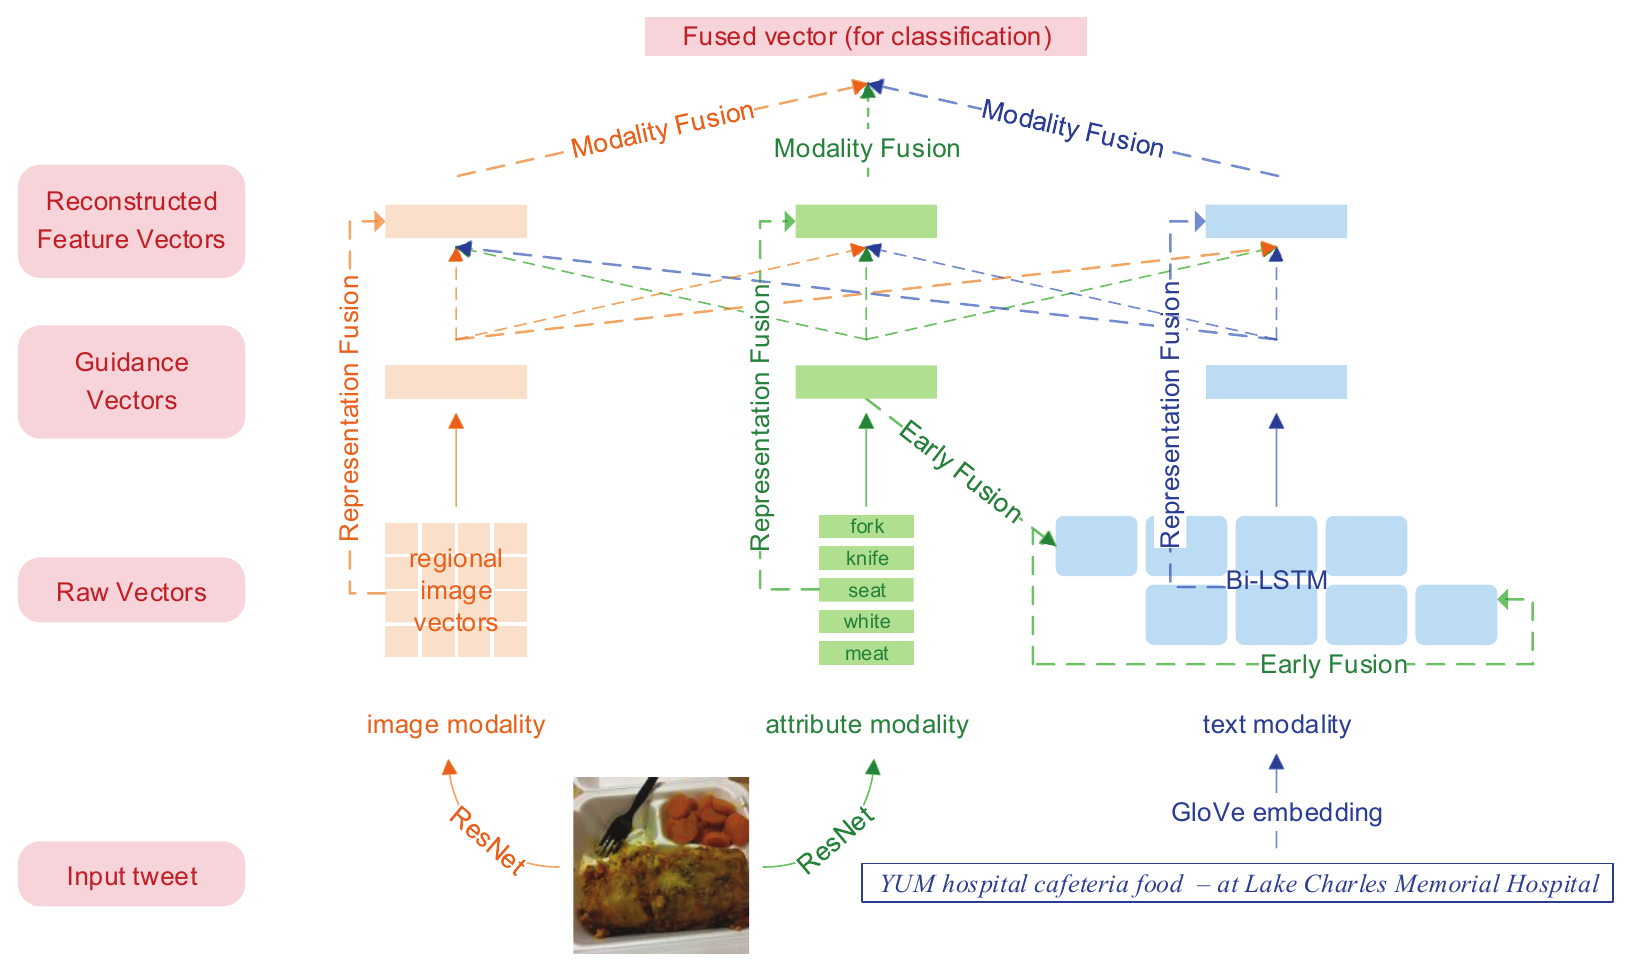
\includegraphics[width=\linewidth]{figures/cai2019_architecture.png}
\end{column}
\begin{column}{0.29\textwidth}
\small
\textbf{Why this paper?}
\begin{itemize}
  \item Explicit interaction, not just concatenation.
  \item Attribute path can be changed independently.
\end{itemize}
\begin{block}{Published F1}
HFM: \textbf{80.18\%}\\
Concat3: 78.74\%\\[1mm]
\textbf{+1.44 points}
\end{block}
\end{column}
\end{columns}
\vfill
{\scriptsize Figure: Cai et al., ACL 2019, Fig.~2; also reproduced in the project report.}
\end{frame}

\begin{frame}{Reproduction: similar score, smaller advantage}
\begin{center}
\begin{tabular}{lcc}
\toprule
 & Published F1 & Local F1 \\
\midrule
Three-way concatenation & 78.74 & $79.90\pm0.49$ \\
Hierarchical fusion & 80.18 & $\mathbf{80.16\pm0.78}$ \\
\bottomrule
\end{tabular}
\end{center}
\begin{itemize}
  \item Local models share regional image features and COCO attributes.
  \item HFM leads in all three seeds, but only by \textbf{about 0.27 points}.
  \item Matching the absolute score does \textbf{not} recover the full gain.
\end{itemize}
\vfill
{\scriptsize Local results: mean $\pm$ sample SD, three seeds; positive-class test F1 (\%).\\
Pipeline-level PyTorch reproduction; visual preparation and training differ from the original.}
\end{frame}

\begin{frame}{Improvement: change the words, not the fusion}
\small
\textbf{Why?} Object-level attributes may describe what is visible,\\
but fail to represent the meaning relevant to sarcasm.

\begin{columns}[c,onlytextwidth]
\begin{column}{0.34\textwidth}
\includegraphics[width=\linewidth,height=2.9cm,keepaspectratio]{data/raw/dataset_image/682716753374351360.jpg}
\end{column}
\begin{column}{0.63\textwidth}
\begin{block}{Actual filtered example}
\textbf{Predicted:} glass, holding, wine, person, drink
\end{block}
These words capture the objects, \textbf{not the dark joke}.\\
I tested richer attributes with affective context.
\end{column}
\end{columns}

\begin{block}{My improvement}
Use CLIP to select image attributes that also include affective context,\\
without redesigning the fusion model.
\end{block}
\vfill
{\scriptsize Test example: local COCO predictor with stopword filtering, ID 682716753374351360;\\
saved output in \texttt{notebooks/resnet101\_coco\_attributes\_filtered.ipynb}.}
\end{frame}

\begin{frame}{The idea: match the image to candidate phrases}
\begin{block}{How CLIP is used}
Compare the image with phrases such as:
\end{block}
\begin{itemize}
  \item ``a photo of wine.''
  \item ``a photo of a scene that feels sad.''
\end{itemize}
\vspace{3mm}
Use the matching words as image attributes for the \textbf{same fusion model}.

\textbf{What changes?} How the image attributes are selected, not the fusion.
\vfill
{\scriptsize Illustrative phrases, not measured matches for the wine image. CLIP never reads the tweet.}
\end{frame}

\begin{frame}{Main result: a small, inconsistent gain}
\begin{center}
\begin{tabular}{lc}
\toprule
Model & Test F1 (\%) \\
\midrule
Reproduced HFM & $80.16\pm0.78$ \\
HFM with sentiment-aware CLIP & $\mathbf{80.32\pm0.38}$ \\
\bottomrule
\end{tabular}
\end{center}
\begin{itemize}
  \item Mean F1 improved by only \textbf{0.16 points}.
  \item The gain was \textbf{not consistent across seeds}; accuracy was slightly lower.
\end{itemize}
\begin{block}{Takeaway}
Changing the attributes produced a small average F1 gain,\\
but not a reliable overall improvement over the baseline.
\end{block}
{\scriptsize Mean $\pm$ sample SD, three classifier seeds on MMSD. No statistical significance claim.}
\end{frame}

\end{document}
